\section{Capítulo 4 -- Pilhas e Filas}

A lista encadeada do Capítulo 3 permite inserir e remover em qualquer ponto. Muitos problemas, porém, precisam do contrário: de uma estrutura que \textbf{restringe} onde se pode inserir e remover. Essas restrições não são uma limitação, e sim uma garantia de ordem. Neste capítulo você vai construir as duas estruturas restritas mais usadas da computação: a \textbf{pilha} e a \textbf{fila}. Ambas serão genéricas, com templates (Capítulo 1), e construídas com nós encadeados (Capítulo 3).

\subsection{4.1 Estruturas com regras de acesso}

Pense em uma pilha de pratos: você coloca um prato sempre em cima e, quando precisa de um, pega o de cima. O último prato colocado é o primeiro a ser usado. Agora pense na fila de um banco: quem chega vai para o final, e quem é atendido sai pela frente. O primeiro a chegar é o primeiro a sair.

Essas duas regras têm nomes:

\begin{itemize}
  \item \textbf{LIFO} (\textit{Last In, First Out}, o último a entrar é o primeiro a sair): é a regra da \textbf{pilha}.
  \item \textbf{FIFO} (\textit{First In, First Out}, o primeiro a entrar é o primeiro a sair): é a regra da \textbf{fila}.
\end{itemize}

Você usa as duas o tempo todo, mesmo sem perceber. O botão de desfazer (Ctrl+Z) de um editor é uma pilha: desfaz primeiro a última ação. Os documentos enviados para uma impressora formam uma fila: são impressos na ordem em que chegaram.

\subsection{4.2 A pilha}

Em uma pilha, todas as operações acontecem em uma única ponta, chamada \textbf{topo}.

\begin{center}
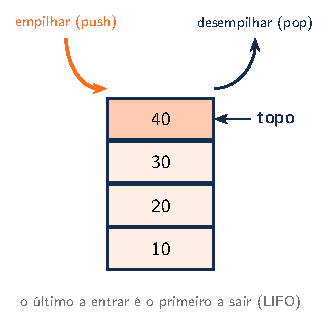
\includegraphics[width=0.6\linewidth,keepaspectratio]{imagens/capitulo-04_pilha.pdf}
\end{center}

\begin{center}
\begin{tabular}{@{}p{0.3\linewidth}p{0.42\linewidth}p{0.14\linewidth}@{}}
\toprule
\rowcolor{headergray}
\tblheader{Operação} & \tblheader{O que faz} & \tblheader{Custo} \\
\midrule
\texttt{empilhar(v)} & coloca \texttt{v} no topo (\textit{push}) & $O(1)$ \\
\rowcolor{rowgray} \texttt{desempilhar()} & retira e devolve o topo (\textit{pop}) & $O(1)$ \\
\texttt{espiar()} & devolve o topo sem retirar (\textit{top}) & $O(1)$ \\
\rowcolor{rowgray} \texttt{vazia()} & diz se não há elementos & $O(1)$ \\
\texttt{quantidade()} & quantos elementos há & $O(1)$ \\
\bottomrule
\end{tabular}
\end{center}

\subsection{4.3 Pilha com nós encadeados}

Na lista encadeada, inserir e remover no \textbf{início} custa $O(1)$. Então basta usar o início da lista como topo da pilha: empilhar é inserir no início, desempilhar é remover do início. Cada nó aponta para o que está \textbf{abaixo} dele.

Repare em duas novidades. O nó agora fica \textbf{dentro} da classe, porque só a pilha precisa conhecê-lo. E desempilhar uma pilha vazia é um erro de quem chama: em vez de devolver um valor inventado, a função \textbf{lança uma exceção} com \texttt{throw}, que interrompe a operação e pode ser tratada com \texttt{try}/\texttt{catch}.

\begin{codigo}
\begin{Verbatim}[breaklines=true, breaksymbolleft={}, fontsize=\footnotesize]
#include <stdexcept>   // runtime_error

template <typename T>
class Pilha {
private:
    struct No {
        T valor;
        No *abaixo;    // o nó que está embaixo deste
    };
    No *topo = nullptr;
    int tamanho = 0;

public:
    Pilha() = default;
    ~Pilha() {
        while (!vazia()) {
            desempilhar();
        }
    }
    Pilha(const Pilha &) = delete;
    Pilha &operator=(const Pilha &) = delete;

    bool vazia() const { return topo == nullptr; }
    int quantidade() const { return tamanho; }

    void empilhar(const T &valor) {
        topo = new No{valor, topo};   // o novo nó fica por cima do antigo topo
        tamanho++;
    }

    T desempilhar() {
        if (vazia()) {
            throw runtime_error("pilha vazia");
        }
        No *velho = topo;
        T valor = velho->valor;
        topo = topo->abaixo;
        delete velho;
        tamanho--;
        return valor;
    }

    const T &espiar() const {
        if (vazia()) {
            throw runtime_error("pilha vazia");
        }
        return topo->valor;
    }
};

int main() {
    Pilha<int> p;
    for (int v = 10; v <= 40; v += 10) {
        p.empilhar(v);                       // 10, 20, 30, 40
    }
    cout << "Topo: " << p.espiar() << endl;  // 40
    cout << p.desempilhar() << endl;         // 40
    cout << p.desempilhar() << endl;         // 30
    cout << "Restam " << p.quantidade() << endl;  // 2

    Pilha<string> vazia;
    try {
        vazia.desempilhar();
    } catch (const runtime_error &erro) {
        cout << "Erro: " << erro.what() << endl;  // Erro: pilha vazia
    }
}
\end{Verbatim}
\end{codigo}

Como a classe é um template, a mesma pilha serve para \texttt{int}, \texttt{string}, \texttt{char} ou qualquer outro tipo. Todas as operações são $O(1)$: nenhuma percorre a estrutura.

\subsection{4.4 Aplicações da pilha}

\subsubsection{Verificar se os parênteses estão balanceados}

Compiladores e editores de código precisam conferir se cada \texttt{(}, \texttt{[} e \texttt{\{} foi fechado na ordem certa. A expressão \texttt{\{[(2+3)*4]\}} está correta; \texttt{(2+3]} e \texttt{((1+2)} não estão.

A pilha resolve isso de forma natural: cada símbolo que abre é empilhado; cada símbolo que fecha precisa combinar com o topo. O último aberto deve ser o primeiro fechado, exatamente a regra LIFO.

\begin{codigo}
\begin{Verbatim}[breaklines=true, breaksymbolleft={}, fontsize=\footnotesize]
// trecho: usa a classe Pilha da seção 4.3
bool balanceado(const string &expressao) {
    Pilha<char> abertos;
    for (char c : expressao) {
        if (c == '(' || c == '[' || c == '{') {
            abertos.empilhar(c);
        } else if (c == ')' || c == ']' || c == '}') {
            if (abertos.vazia()) {
                return false;                 // fechou algo que não foi aberto
            }
            char a = abertos.desempilhar();
            if ((c == ')' && a != '(') || (c == ']' && a != '[') || (c == '}' && a != '{')) {
                return false;                 // fechou com o tipo errado
            }
        }
    }
    return abertos.vazia();                   // sobrou algo aberto?
}
\end{Verbatim}
\end{codigo}

\subsubsection{Calcular expressões em notação pós-fixa}

Na notação que usamos no dia a dia, o operador fica entre os números: $(3 + 4) \cdot 2$. Na \textbf{notação pós-fixa}, o operador vem depois dos operandos: \texttt{3 4 + 2 *}. Ela dispensa parênteses e é muito fácil de calcular com uma pilha, por isso calculadoras e compiladores a usam internamente.

A regra é: número, empilha; operador, desempilha dois números, faz a conta e empilha o resultado. No final, o resultado é o único valor na pilha.

\begin{center}
\begin{tabular}{@{}p{0.16\linewidth}p{0.42\linewidth}p{0.28\linewidth}@{}}
\toprule
\rowcolor{headergray}
\tblheader{Lido} & \tblheader{Ação} & \tblheader{Pilha (topo à direita)} \\
\midrule
\texttt{3} & empilha & 3 \\
\rowcolor{rowgray} \texttt{4} & empilha & 3 4 \\
\texttt{+} & desempilha 4 e 3, empilha 3 + 4 & 7 \\
\rowcolor{rowgray} \texttt{2} & empilha & 7 2 \\
\texttt{*} & desempilha 2 e 7, empilha 7 $\cdot$ 2 & 14 \\
\bottomrule
\end{tabular}
\end{center}

\begin{codigo}
\begin{Verbatim}[breaklines=true, breaksymbolleft={}, fontsize=\footnotesize]
// trecho: usa a classe Pilha da seção 4.3
#include <sstream>   // istringstream: lê a expressão palavra por palavra

double avaliarPosfixa(const string &expressao) {
    Pilha<double> p;
    istringstream entrada(expressao);
    string item;
    while (entrada >> item) {
        if (item == "+" || item == "-" || item == "*" || item == "/") {
            double b = p.desempilhar();   // o segundo operando sai primeiro
            double a = p.desempilhar();
            if (item == "+") p.empilhar(a + b);
            else if (item == "-") p.empilhar(a - b);
            else if (item == "*") p.empilhar(a * b);
            else p.empilhar(a / b);
        } else {
            p.empilhar(stod(item));       // converte o texto em número
        }
    }
    return p.desempilhar();
}
\end{Verbatim}
\end{codigo}

Veja as duas aplicações funcionando juntas. Para o programa ficar mais curto, a pilha aparece em versão resumida, só com as operações usadas aqui:

\begin{codigo}
\begin{Verbatim}[breaklines=true, breaksymbolleft={}, fontsize=\footnotesize]
#include <stdexcept>
#include <sstream>

template <typename T>
class Pilha {
private:
    struct No {
        T valor;
        No *abaixo;
    };
    No *topo = nullptr;

public:
    Pilha() = default;
    ~Pilha() { while (!vazia()) desempilhar(); }
    Pilha(const Pilha &) = delete;
    Pilha &operator=(const Pilha &) = delete;

    bool vazia() const { return topo == nullptr; }
    void empilhar(const T &valor) { topo = new No{valor, topo}; }
    T desempilhar() {
        if (vazia()) throw runtime_error("pilha vazia");
        No *velho = topo;
        T valor = velho->valor;
        topo = topo->abaixo;
        delete velho;
        return valor;
    }
};

bool balanceado(const string &expressao) {
    Pilha<char> abertos;
    for (char c : expressao) {
        if (c == '(' || c == '[' || c == '{') {
            abertos.empilhar(c);
        } else if (c == ')' || c == ']' || c == '}') {
            if (abertos.vazia()) {
                return false;
            }
            char a = abertos.desempilhar();
            if ((c == ')' && a != '(') || (c == ']' && a != '[') || (c == '}' && a != '{')) {
                return false;
            }
        }
    }
    return abertos.vazia();
}

double avaliarPosfixa(const string &expressao) {
    Pilha<double> p;
    istringstream entrada(expressao);
    string item;
    while (entrada >> item) {
        if (item == "+" || item == "-" || item == "*" || item == "/") {
            double b = p.desempilhar();
            double a = p.desempilhar();
            if (item == "+") p.empilhar(a + b);
            else if (item == "-") p.empilhar(a - b);
            else if (item == "*") p.empilhar(a * b);
            else p.empilhar(a / b);
        } else {
            p.empilhar(stod(item));
        }
    }
    return p.desempilhar();
}

int main() {
    cout << boolalpha;
    cout << balanceado("{[(2+3)*4]}") << endl;   // true
    cout << balanceado("(2+3]") << endl;         // false
    cout << balanceado("((1+2)") << endl;        // false
    cout << balanceado(")(") << endl;            // false

    cout << avaliarPosfixa("3 4 + 2 *") << endl;          // 14
    cout << avaliarPosfixa("5 1 2 + 4 * + 3 -") << endl;  // 14
}
\end{Verbatim}
\end{codigo}

\subsubsection{A pilha de execução}

Você já conhece uma pilha muito importante: a \textbf{pilha de execução} do programa, citada nos Capítulos 1 e 2. Cada vez que uma função é chamada, um espaço com suas variáveis é empilhado; quando a função termina, esse espaço é desempilhado e o programa volta ao ponto em que estava. Por isso uma recursão sem fim causa o erro conhecido como \textit{stack overflow} (estouro da pilha): as chamadas são empilhadas até não caber mais nenhuma.

\subsection{4.5 A fila}

Em uma fila, os elementos entram por uma ponta (o \textbf{fim}) e saem pela outra (o \textbf{início}).

\begin{center}
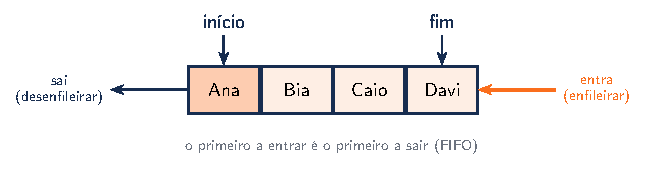
\includegraphics[width=0.85\linewidth,keepaspectratio]{imagens/capitulo-04_fila.pdf}
\end{center}

\begin{center}
\begin{tabular}{@{}p{0.3\linewidth}p{0.42\linewidth}p{0.14\linewidth}@{}}
\toprule
\rowcolor{headergray}
\tblheader{Operação} & \tblheader{O que faz} & \tblheader{Custo} \\
\midrule
\texttt{enfileirar(v)} & coloca \texttt{v} no fim (\textit{enqueue}) & $O(1)$ \\
\rowcolor{rowgray} \texttt{desenfileirar()} & retira e devolve o início (\textit{dequeue}) & $O(1)$ \\
\texttt{frente()} & devolve o início sem retirar & $O(1)$ \\
\rowcolor{rowgray} \texttt{vazia()} & diz se não há elementos & $O(1)$ \\
\bottomrule
\end{tabular}
\end{center}

\subsection{4.6 Fila com nós encadeados}

A lista encadeada com ponteiro para o fim (Capítulo 3) já tem tudo que a fila precisa: inserir no fim e remover do início, ambos em $O(1)$.

\begin{codigo}
\begin{Verbatim}[breaklines=true, breaksymbolleft={}, fontsize=\footnotesize]
#include <stdexcept>

template <typename T>
class Fila {
private:
    struct No {
        T valor;
        No *proximo;
    };
    No *inicio = nullptr;   // de onde sai
    No *fim = nullptr;      // por onde entra
    int tamanho = 0;

public:
    Fila() = default;
    ~Fila() {
        while (!vazia()) {
            desenfileirar();
        }
    }
    Fila(const Fila &) = delete;
    Fila &operator=(const Fila &) = delete;

    bool vazia() const { return inicio == nullptr; }
    int quantidade() const { return tamanho; }

    void enfileirar(const T &valor) {
        No *novo = new No{valor, nullptr};
        if (fim == nullptr) {
            inicio = novo;          // fila vazia: o novo é o primeiro
        } else {
            fim->proximo = novo;    // entra atrás do último
        }
        fim = novo;
        tamanho++;
    }

    T desenfileirar() {
        if (vazia()) {
            throw runtime_error("fila vazia");
        }
        No *velho = inicio;
        T valor = velho->valor;
        inicio = inicio->proximo;
        if (inicio == nullptr) {
            fim = nullptr;          // a fila ficou vazia
        }
        delete velho;
        tamanho--;
        return valor;
    }

    const T &frente() const {
        if (vazia()) {
            throw runtime_error("fila vazia");
        }
        return inicio->valor;
    }
};

int main() {
    Fila<string> atendimento;
    atendimento.enfileirar("Ana");
    atendimento.enfileirar("Bia");
    atendimento.enfileirar("Caio");

    cout << "Proximo a ser atendido: " << atendimento.frente() << endl;  // Ana
    while (!atendimento.vazia()) {
        cout << "Atendendo " << atendimento.desenfileirar() << endl;     // Ana, Bia, Caio
    }
}
\end{Verbatim}
\end{codigo}

Repare no cuidado em \texttt{desenfileirar}: quando o último elemento sai, \texttt{fim} também precisa voltar a \texttt{nullptr}. Se isso for esquecido, o próximo \texttt{enfileirar} vai ligar o novo nó a um nó que já foi apagado.

\subsection{4.7 Fila circular em vetor}

Também é possível fazer uma fila com um vetor de tamanho fixo, o que evita alocar um nó a cada inserção. A ideia ingênua seria remover sempre da posição 0 e deslocar os demais elementos, mas isso custaria $O(n)$ a cada saída.

A solução é a \textbf{fila circular}: em vez de mover os elementos, movemos os índices. \texttt{inicio} indica onde está o primeiro elemento e \texttt{fim} indica onde entra o próximo. Quando um índice passa da última posição, ele volta para a posição 0, como se o vetor fosse um anel. Quem faz essa volta é o operador de resto da divisão, \texttt{\%}.

\begin{center}
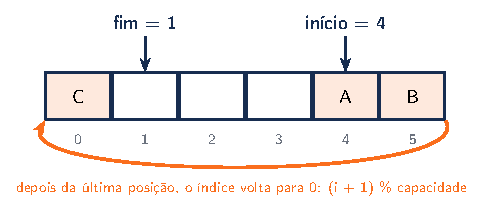
\includegraphics[width=0.9\linewidth,keepaspectratio]{imagens/capitulo-04_fila_circular.pdf}
\end{center}

Na figura, a fila tem capacidade 6 e contém, na ordem de saída, A (posição 4), B (posição 5) e C (posição 0). O próximo elemento entrará na posição 1.

\begin{codigo}
\begin{Verbatim}[breaklines=true, breaksymbolleft={}, fontsize=\footnotesize]
#include <stdexcept>

template <typename T>
class FilaCircular {
private:
    T *dados;
    int capacidade;
    int inicio = 0;    // posição do primeiro elemento
    int fim = 0;       // posição onde entra o próximo
    int tamanho = 0;

public:
    explicit FilaCircular(int cap) : dados(new T[cap]), capacidade(cap) {}
    ~FilaCircular() { delete[] dados; }
    FilaCircular(const FilaCircular &) = delete;
    FilaCircular &operator=(const FilaCircular &) = delete;

    bool vazia() const { return tamanho == 0; }
    bool cheia() const { return tamanho == capacidade; }

    bool enfileirar(const T &valor) {
        if (cheia()) {
            return false;                     // não há espaço
        }
        dados[fim] = valor;
        fim = (fim + 1) % capacidade;         // depois da última, volta para 0
        tamanho++;
        return true;
    }

    T desenfileirar() {
        if (vazia()) {
            throw runtime_error("fila vazia");
        }
        T valor = dados[inicio];
        inicio = (inicio + 1) % capacidade;
        tamanho--;
        return valor;
    }
};

int main() {
    FilaCircular<int> f(6);
    for (int v = 1; v <= 6; v++) {
        f.enfileirar(v);                         // ocupa as posições 0 a 5
    }
    cout << boolalpha << f.enfileirar(7) << endl;  // false: está cheia

    cout << f.desenfileirar() << " ";            // 1
    cout << f.desenfileirar() << endl;           // 2

    f.enfileirar(7);                             // entra na posição 0 (deu a volta)
    f.enfileirar(8);                             // entra na posição 1
    while (!f.vazia()) {
        cout << f.desenfileirar() << " ";        // 3 4 5 6 7 8
    }
    cout << endl;
}
\end{Verbatim}
\end{codigo}

A fila circular faz todas as operações em $O(1)$ e não aloca memória a cada inserção, mas tem capacidade fixa. É muito usada em sistemas que recebem dados continuamente, como teclados, placas de rede e players de áudio, onde é chamada de \textit{buffer} circular.

\subsection{4.8 Aplicações da fila}

\begin{itemize}
  \item \textbf{Atendimento por ordem de chegada}: senhas de banco, pedidos de uma lanchonete, chamados de suporte.
  \item \textbf{Fila de impressão}: os documentos são impressos na ordem em que foram enviados.
  \item \textbf{Escalonamento de processos}: o sistema operacional reveza o processador entre os programas usando filas.
  \item \textbf{Busca em largura em grafos}: no Capítulo 6, a fila vai garantir que um grafo seja explorado em camadas, primeiro os vizinhos mais próximos.
\end{itemize}

\subsection{4.9 Pilhas e filas prontas}

A biblioteca padrão do C++ oferece \texttt{stack} (pilha), \texttt{queue} (fila) e \texttt{deque}, uma fila de duas pontas que permite inserir e remover no início e no fim. Atenção a um detalhe: no C++, \texttt{pop()} retira o elemento, mas \textbf{não o devolve}. Para ler o valor, use \texttt{top()} (pilha) ou \texttt{front()} (fila) antes de chamar \texttt{pop()}.

\begin{codigo}
\begin{Verbatim}[breaklines=true, breaksymbolleft={}, fontsize=\footnotesize]
#include <stack>
#include <queue>

int main() {
    stack<int> pilha;
    pilha.push(10);
    pilha.push(20);
    cout << pilha.top() << endl;    // 20: lê o topo
    pilha.pop();                    // retira, sem devolver

    queue<string> fila;
    fila.push("Ana");
    fila.push("Bia");
    cout << fila.front() << endl;   // Ana: lê o início
    fila.pop();
    cout << fila.size() << endl;    // 1
}
\end{Verbatim}
\end{codigo}

\begin{destaque}{Comparando com Python}
Em Python, a própria \texttt{list} funciona bem como pilha, porque \texttt{append} e \texttt{pop} no fim custam $O(1)$. Para fila, porém, \textbf{não} use a lista: \texttt{lista.pop(0)} desloca todos os elementos e custa $O(n)$. Use o \texttt{deque}:

\begin{codigo}
\begin{Verbatim}[breaklines=true, breaksymbolleft={}, fontsize=\footnotesize]
from collections import deque

pilha = []
pilha.append(10)
pilha.append(20)
print(pilha.pop())        # 20, O(1)

fila = deque()
fila.append("Ana")        # enfileirar, O(1)
fila.append("Bia")
print(fila.popleft())     # Ana, desenfileirar em O(1)
\end{Verbatim}
\end{codigo}
\end{destaque}

\subsection{Erros Comuns}

\begin{itemize}
  \item \textbf{Desempilhar ou desenfileirar uma estrutura vazia.} Sempre verifique \texttt{vazia()} antes, ou trate a exceção. Na STL do C++, chamar \texttt{top()} ou \texttt{pop()} em uma pilha vazia tem comportamento indefinido.
  \item \textbf{Esperar que o \texttt{pop()} da STL devolva o valor.} Ele só retira. Leia com \texttt{top()} ou \texttt{front()} antes.
  \item \textbf{Inverter a ordem dos operandos.} Na pós-fixa, o primeiro valor desempilhado é o \textit{segundo} operando: em \texttt{8 2 -}, a conta é $8 - 2$, não $2 - 8$.
  \item \textbf{Não zerar o \texttt{fim} quando a fila esvazia.} Ao retirar o último elemento, \texttt{fim} deve voltar a \texttt{nullptr}.
  \item \textbf{Esquecer o resto da divisão na fila circular.} Sem \texttt{\% capacidade}, o índice passa do fim do vetor e o programa escreve fora da memória reservada.
  \item \textbf{Confundir fila cheia com fila vazia.} Na fila circular, \texttt{inicio == fim} acontece nos dois casos. Por isso guardamos o \texttt{tamanho}.
  \item \textbf{Usar \texttt{lista.pop(0)} como fila em Python.} Cada saída custa $O(n)$; com muitos elementos, o programa fica lento. Use \texttt{deque}.
\end{itemize}
